% Please use the skeleton file you have received in the
% invitation-to-submit email, where your data are already
% filled in. Otherwise please make sure you insert your
% data according to the instructions in PoSauthmanual.pdf
\documentclass{PoS}

\title{Summary of Working Group 4 : mixing and mixing-related $CP$ violation in the $B$ system}

\ShortTitle{All SM everything}

\author{\speaker{Alessandro Gaz}\\
        Nagoya\\
        E-mail: \email{gaz@hepl.phys.nagoya-u.ac.jp}\\
        \speaker{Vladimir V. Gligorov}\thanks{I would like to thank my mum, dad, and trade union representative for their support. Couldn't have done it without you!}\\
        LPNHE, Universit\'{e} Pierre et Marie Curie, Universit\'{e} Paris Diderot, CNRS/IN2P3, Paris, France\\
        E-mail: \email{vgligoro@lpnhe.in2p3.fr}\\
        \speaker{Dean Robinson}\\
        Cincinnati\\
        E-mail: \email{dean.robinson@uc.edu}\\
        }

%\author{Another Author\\
%        Affiliation\\
%        E-mail: \email{...}}

\abstract{$B$ mesons mix and in mixing do wonderful and amazing things.}

\FullConference{9th International Workshop on the CKM Unitarity Triangle\\
		28  November - 3 December 2016\\
		Tata Institute for Fundamental Research (TIFR), Mumbai, India}


\begin{document}

\section{Introduction}
Neutral beauty mesons can oscillate into their antiparticles through the exchange of $W^\pm W^\mp$ pairs, so that the 
physical states (those with well defined masses and lifetimes) are admixtures of the flavour eigenstates. This gives
rise to both mass ($\delta m_{(d,s)}$) and width ($\Delta\Gamma_{(d,s)}$) splittings in the $B^0_d$ and $B^0_s$ systems, as well
as two types of related $CP$ violation. The first, $CP$ violation in mixing, occurs when the meson and antimeson have different
probablities to oscillate into each other, and is predicted to be very close to zero in the Standard Model (SM) with a very
small theoretical uncertainty. The second, $CP$ violation in the intereference of decay and mixing, occurs when both the meson
and antimeson can decay to the final state, and the decay paths with and without intermediate mixing interfere. This kind of $CP$
violation is highly sensitive to the imaginary component of the CKM matrix and its absolute size depends on the final state in question.

Aside from their intrinsically fundamental nature, measurements of mass and width splittings and mixing-related $CP$ violation are
of great interest because many of the observables can be predicted very precisely in the SM, and because new particles or force-carriers
beyond the SM (BSM) can alter these predictions in experimentally observable ways. Many different experimental collaborations have contributed
to our understanding of mixing in the $B$ system, from the inital discovery of $B$ mixing by the ARGUS collaboration~\cite{}, to precise measurements
of $\delta m_{(d,s)}$ and the CKM-angles $\alpha$ and $\beta$ at the b-factories and Tevatron~\cite{}, to recent precise measurements
of $\phi_s$, $\Delta\Gamma_s$, and first precise mixing-related measurements of the CKM-angle $\gamma$ at ATLAS, CMS, and LHCb~\cite{}. At the same
time, great progress has been made in making more precise theoretical predictions of the SM values of many of these quantities, making
these experimental measurements sensitive probes of BSM physics.

The remainder of this document covers the current status of experimental measurements and theory predictions for each observable of
interest, as well as their near-term outlook. Section~\ref{sec:phisdgs} covers measurements of $\phi_s$ and $\Delta\Gamma_s$, section~\ref{sec:dmdgd} 
mesurements of $\delta m_{(s,d)}$. Section~\ref{sec:photpol} covers the measurements of photon polarization in radiative decays, while
sections~\ref{sec:alpha}~to~\ref{sec:gamma} cover measurements of the CKM angles $\alpha$, $\beta$, and $\gamma$, respectively.
For historical reasons, measurements of $CP$ violation in neutral meson mixing are covered in the proceedings of WG~\cite{}. Finally we conclude,
and discuss the medium to long-term outlook for mixing-related measurements in the $B$ system.




%\section{Measurements of $\phi_s$}


%\section{Measurements of $\Delta\Gamma_{(d,s)}$}

%\section{Measurements of $\Delta m_{(d,s)}$}


% ale: I think it makes more sense to have phi_s and deltaGamma_s in one section:
\section{Measurements of $\phi_s$ and $\Delta\Gamma_s$}
\label{sec:phisdgs}

The $\phi_s$ weak phase and $B^0_s$ meson decay width difference can
be extracted by a time dependent full angular decay analysis of the 
$B^0_s \to J/\psi K^+ K^-$ decays. Such measurements have traditionally
used the subset of decays where the $K^+ K^-$ pair originates in the decay
of a $\phi$ meson, because its narrow width allows for an excellent background
rejection, but since the conference the first measurement which uses
the full $K^+ K^-$ mass spectrum~\cite{LHCbKKHighMass} has become available, and
more such measurements are expected in the future. The importance of
$\phi_s$ is that, in the absence of significant loop-diagram contributions
to $B^0_s \to J/\psi K^+ K^-$ decays (``penguin pollution''),
its value is precisely predicted~\cite{PHISSM} in the SM
\begin{equation}  
\phi_s = -0.036 \pm 0.002 \; ,
\end{equation}
and accurate experimental measurements of $\phi_s$ are therefore 
sensitive probes of the presence of BSM effects in the mixing and decay of $B^0_s$ mesons.

The results that the ATLAS and CMS Experiments obtained on their Run1
datasets using $B^0_s \to J/\psi \phi$ decays are:
\begin{eqnarray}
  \phi_s & = & -0.090 \pm 0.078 (\mbox{stat}) \pm 0.041 (\mbox{syst})\:[\mbox{rad}] \; , \\
  \Delta\Gamma_s & = & \phantom{-}0.085 \pm 0.011 (\mbox{stat}) \pm 0.007 (\mbox{syst})\:[\mbox{ps}^{-1}]  \; ,
\end{eqnarray}
for ATLAS \cite{atlas_phis_8TeV} and:
\begin{eqnarray}
  \phi_s & = & -0.075 \pm 0.097 (\mbox{stat}) \pm 0.031 (\mbox{syst})\:[\mbox{rad}]  \; , \\
  \Delta\Gamma_s & = & \phantom{-}0.095 \pm 0.013 (\mbox{stat}) \pm 0.007 (\mbox{syst})\:[\mbox{ps}^{-1}]  \; ,
\end{eqnarray}
for CMS \cite{cms_phis}. As can be seen in Fig.~\ref{phis_atlas_cms} both measurements are in
excellent agreement with the SM expectations.

\begin{figure}
  \begin{center}
    \begin{tabular}{c c}
      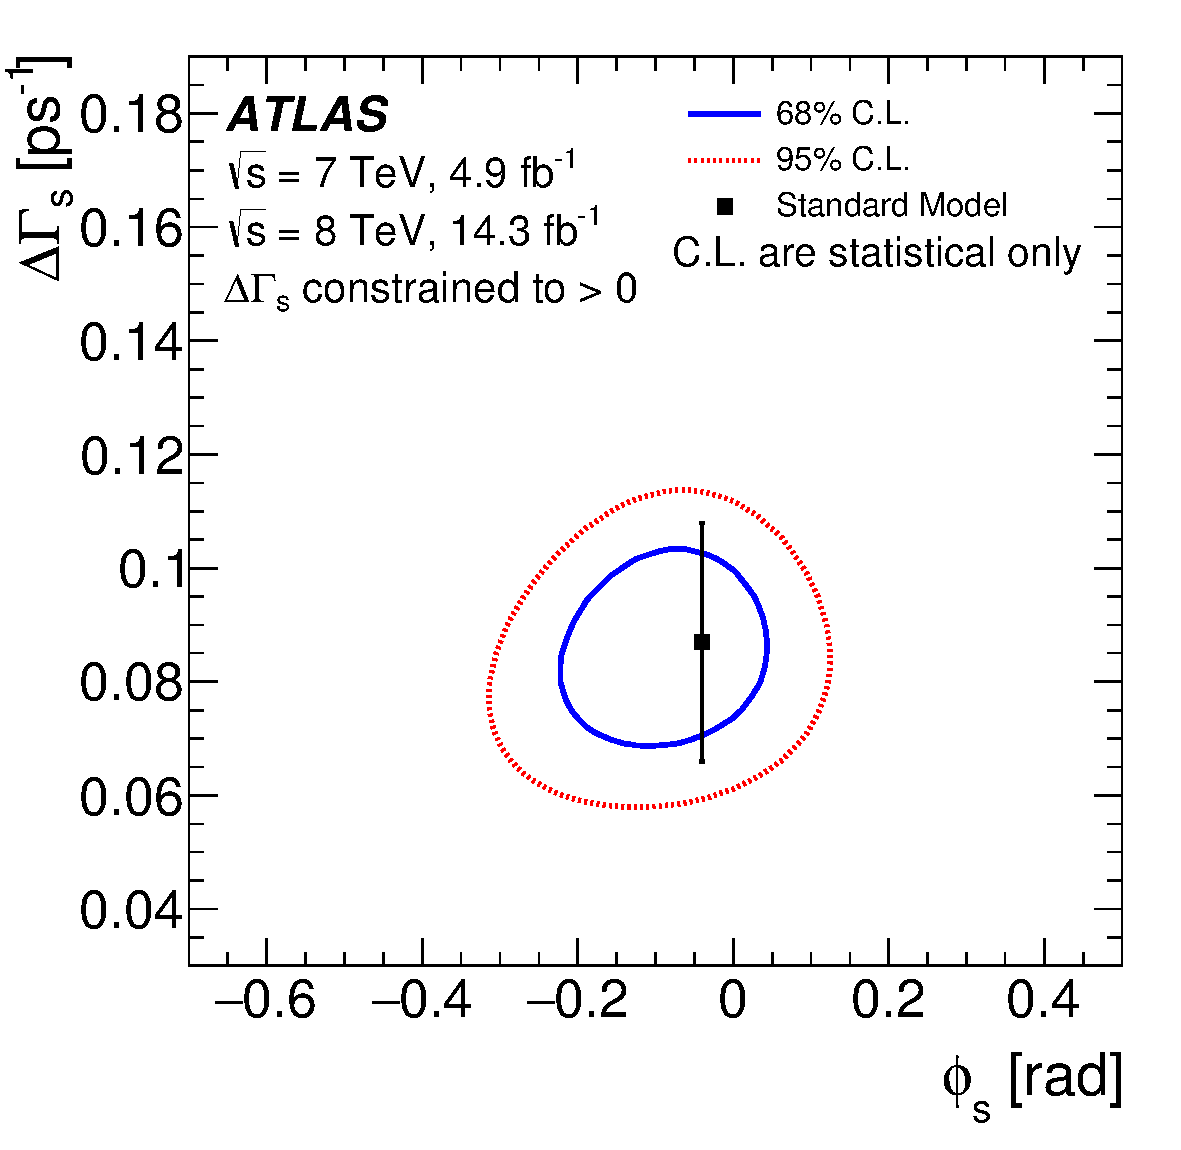
\includegraphics[height=5.5cm]{figs/atlas_phis_result.pdf} &
      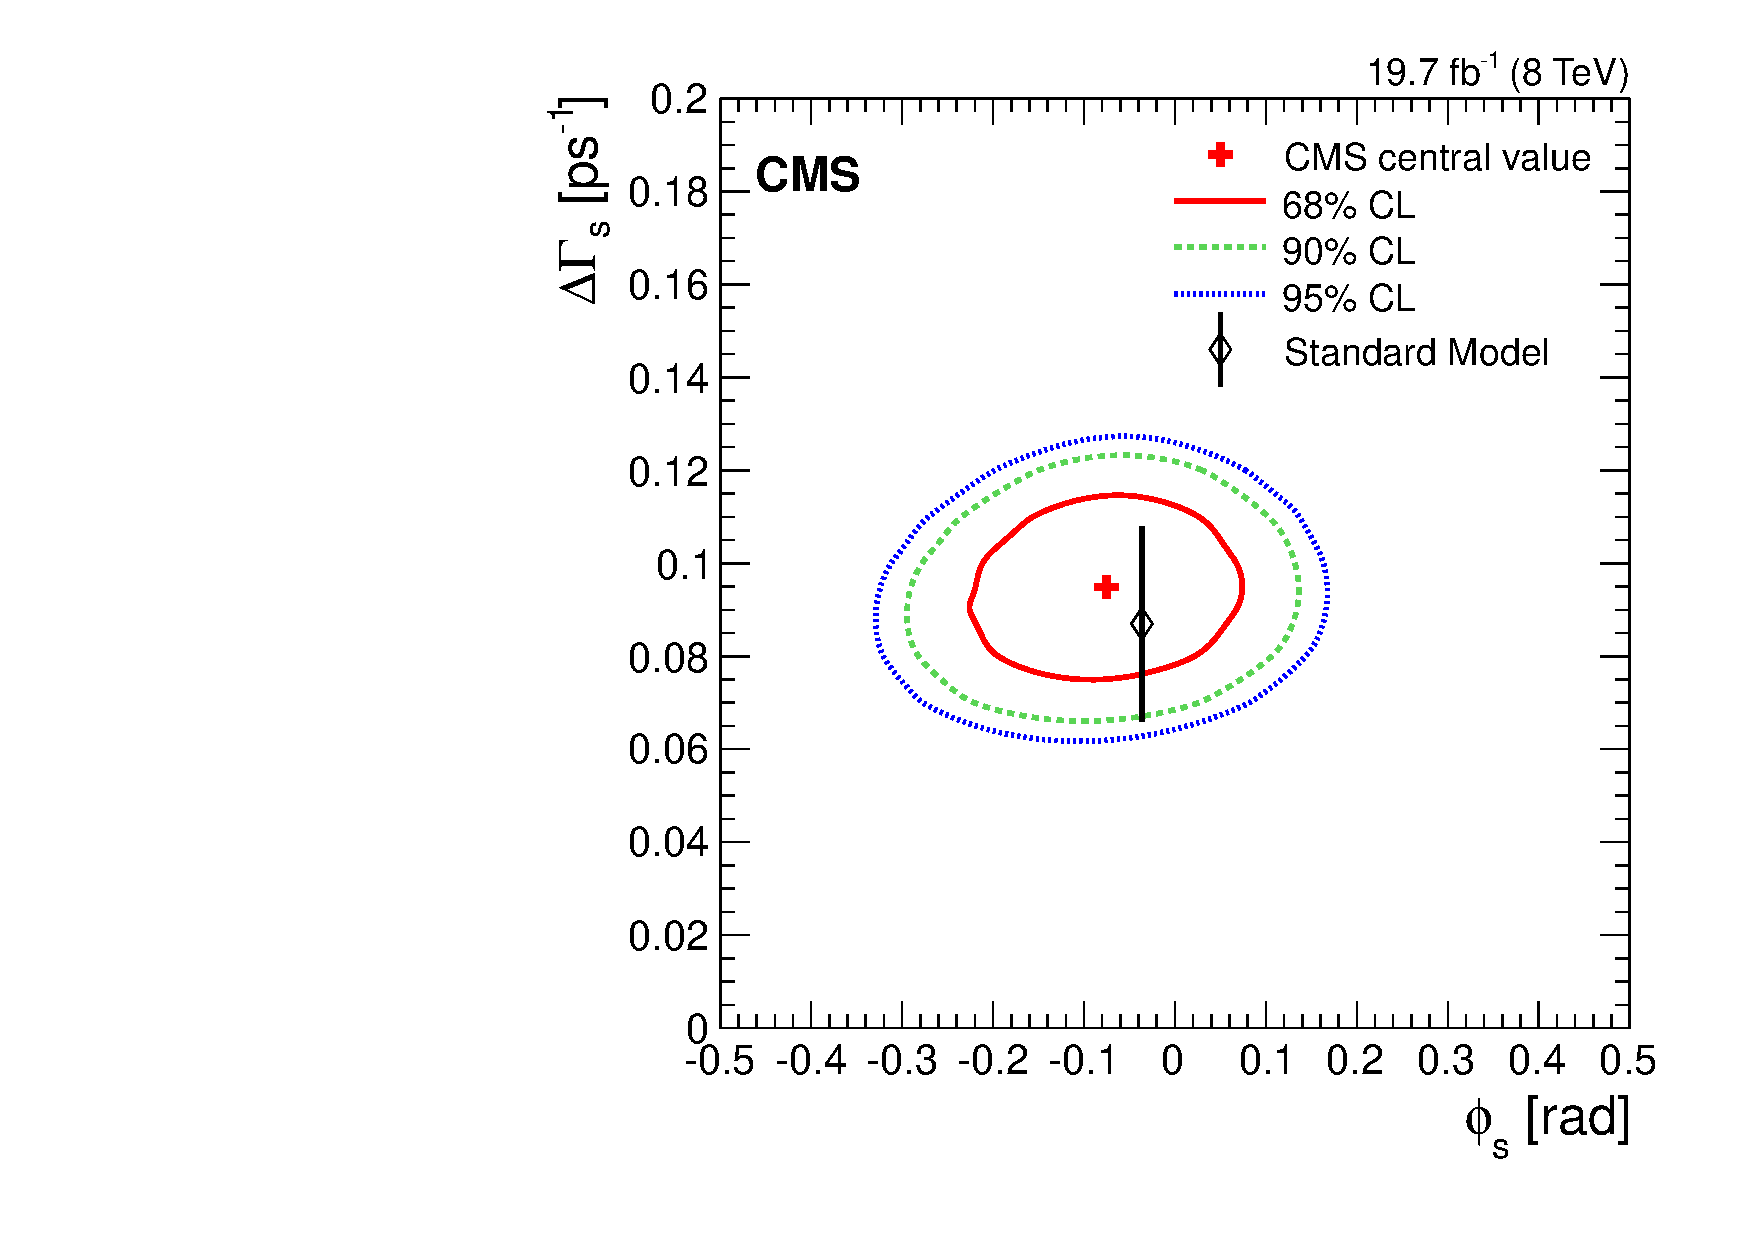
\includegraphics[height=5.5cm]{figs/cms_phis_result.pdf} 
    \end{tabular}
  \end{center}
  \vspace{-0.5cm}
  \caption{\label{phis_atlas_cms}Results on $\phi_s$ and $\Delta\Gamma_s$ from
  $B^0_s \to J/\psi \phi$ decays from (left) ATLAS~\cite{atlas_phis_8TeV} and (right) CMS~\cite{cms_phis}, reproduced from the respective citations.}
\end{figure}

The LHCb measurements of $\phi_s$ are covered in detail elsewhere in these proceedings~\cite{LHCBPHISPROC}.
LHCb uses not only $B^0_s \to J/\psi \phi$ but also $\Bs\to \jpsi\pi^+\pi^-$ decays,
where the $\pi^+\pi^-$ system is dominated by the $f_0(980)$ resonance and is greater than $97.7\%$ \CP-odd.
In this case no angular analysis is required, considerably simplifying the measurement
and providing important complementarity of systematic uncertainties.
The analysis of $B^0_s \to J/\psi \phi$ finds $\Delta\Gamma_s = 0.0805  \pm 0.0091         \pm  0.0032$~ps$^{-1}$,
where the first uncertainty is statistical and the second systematic. 
A combination of $B^0_s \to J/\psi \phi$ and $\Bs\to \jpsi\pi^+\pi^-$ gives $\phis = -0.010  \pm  0.039$~rad, which is the most 
precise single-experiment determination of this quantity.
LHCb has also measured $\phi_s$ using $\Bs\to \psi(2S)\phi$ decays, obtaining
$0.23^{+0.29}_{-0.28} \pm 0.02$ rad.

While $B^0_s \to J/\psi K^+ K^-$ is expected to be dominated by the tree-level diagram,
as the experimental precision on $\phi_s$ improves it will become increasingly important
to account for residual penguin pollution in order to correctly interpret any agreement,
or otherwise, with the theoretical prediction. The size of such effects can be controlled
using a combination of $B^0_s \to J/\psi K^{*0}$ and $B^0 \to J/\psi \rho$ decays,
which are related by U-spin symmetry and in the limit of zero non-factorizable SU(3)
breaking are sensitive to the same, universal, penguin amplitudes and phases.
LHCb has performed measurements of both modes~\cite{LHCb-PAPER-2015-034,LHCb-PAPER-2014-058} and
measures essentially zero penguin pollution to $\phi_s$ with a precision of around 15~mrad
in all three polarization-dependent phases. The LHCb measurement is statistics limited
and penguin pollution to $\phi_s$ should therefore
remain under control as the experimental precision approaches the SM value.

In addition to comparisons with the SM prediction, such tree-dominated measurements of $\phi_s$ can also be compared with the measurement
of the related quantity $\phi_s^{ss\overline{s}}$ in the loop-dominated decays $\Bs \to \phi\phi$ and $\Bs\to \Kp\pi^-\Kp\pi^-$.
In the absence of BSM physics effects, this quantity is expected to be very close to zero.
LHCb has measured~\cite{LHCb-PAPER-2014-026} $\phi_s^{ss\overline{s}} = -0.17 \pm 0.15 \pm 0.03$ rad using
$\Bs\to \phi\phi$, in excellent agreement with the SM prediction. The measurement,
which uses $\Bs\to \Kp\pi^-\Kp\pi^-$, is ongoing; it is considerably more challenging and
requires a two-dimensional Dalitz analysis to account
for the interfering intermediate resonances. 

LHCb has also measured~\cite{LHCb:2017ood} the time-dependent $CP$ violation in $B^0 \to \pi^+ \pi^-$ and $B^0_s \to K^+ K^-$ decays.
These can be interpreted\footnote{In the absence of information about $B^0_s \to K^+ K^-$, measurements of time-dependent $CP$ violation in
$B^0 \to \pi^+ \pi^-$ have traditionally~\cite{HFAG} been combined with other two-body $B^0$ decays in an isospin analysis to obtain a measurement of $\alpha$.}
in a combined U-spin analysis~\cite{Fleischer:1999pa} as either measurements of $\gamma$ or $\phi_s$.
Because the combined U-spin analysis is much less sensitive
to U-spin breaking~\cite{LHCb-PAPER-2014-045} when interpreted as a measurement of $\phi_s$, this is therefore the currently preferred way
to interpret the measurements of these $CP$ observables.

$CP$ violation in $B^0 \to \pi^+ \pi^-$ has been measured previously by BaBar~\cite{Lees:2012mma} and Belle~\cite{Adachi:2013mae},
while the measurement of $B^0_s \to K^+ K^-$ is unique to LHCb. Using a two-dimensional fit to the mass and decay-time
of the neutral $B$ mesons, LHCb observes $CP$ violation in the interference of mixing and decay of $B^0_s$ mesons for the first time, 
and finds
\begin{eqnarray}
C_{\pi\pi}      &=& -0.24 \pm 0.07 \pm 0.01,\phantom{space}
S_{\pi\pi}      = -0.68 \pm 0.06 \pm 0.01,\phantom{space}
\\
C_{KK}      &=& \phantom{+}0.24 \pm 0.06 \pm 0.02,\phantom{space}
S_{KK}      = \phantom{+}0.22 \pm 0.06 \pm 0.02,\phantom{space}
\\
A^{\Delta}_{KK}      &=& -0.75 \pm 0.07 \pm 0.11,\phantom{space}
\end{eqnarray}
where the first uncertainty is statistical and the second systematic. It can be seen that the (co)sinusoidal $C$ and $S$ parameters have
negligible systematic uncertainties, while the hyperbolic $A^{\Delta}_{KK}$, which is sensitive to differences in the distributions
of $B^0_s$ and $\bar{B^0_s}$ induced by $\Delta\Gamma_s$ at high decay-times, is much more sensitive to experimental effects.
This is the most precise single-experiment
determination of $S_{\pi\pi}$, and significantly improves the world-average of this parameter as shown in Fig.~\ref{b2pipiwahfag}.
A combined interpretation in terms of $\phi_s$ is not available at the time of writing but is expected to be performed
in the future, and both LHCb and Belle-II are expected to improve our knowledge of the $CP$ observables in the future. 
The measurement of $A^{\Delta}_{KK}$ is a world first, allowing for a twofold reduction in the ambiguity of the $\phi_s$ determination
and can also be interpreted as a measurement of $\Delta\Gamma_s$.

\begin{figure}
  \begin{center}
    \begin{tabular}{c c}
      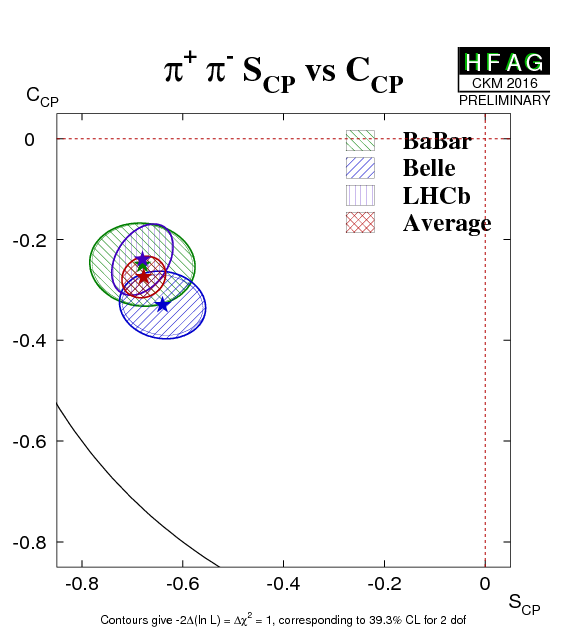
\includegraphics[height=7.5cm]{figs/pi+pi-S_CPvsC_CP.png} &
    \end{tabular}
  \end{center}
  \vspace{-0.5cm}
  \caption{\label{b2pipiwahfag}World average of time-dependent $CP$ observables in $B^0 \to \pi^+ \pi^-$, reproduced from HFAG~\cite{HFAG}.}
\end{figure}

% and one section for Deltam_d,s and DeltaGamma_d:
\section{Measurements of $\Delta m_{(d,s)}$ and $\Delta\Gamma_d$}
\label{sec:dmdgd}

The neutral $B$ meson mass splittings $\Delta m_{(d,s)}$ have been precisely measured by BaBar, Belle, CDF, D0, and LHCb.
The world average~\cite{HFAG} of these measurements is currently dominated by the LHCb determinations,
based on an analysis~\cite{LHCb-PAPER-2015-031} of semileptonic $B^0$ decays in the case of $\Delta m_d$, and based on an analysis~\cite{LHCb-PAPER-2013-006} of $B^0_s \to \D^-_s \pi^+$ decays
in the case of $\Delta m_s$. LHCb finds
\begin{equation}
\Delta m_d = (0.505 \pm 0.0021 \pm 0.0010) \textrm{ps}^{-1}\,,\phantom{space} 
\Delta m_s = (17.768 \pm 0.023 \pm 0.006) \textrm{ps}^{-1}
\end{equation}
where the first uncertainty is statistical, and the second systematic. Neither analysis is systematics limited,
and LHCb is expected to update both measurements in the future. Belle-II will also be able to make a significant contribution
to a precise measurement of $\Delta m_d$. A measurement of $\Delta m_s$ will be difficult for ATLAS and CMS because of a lack of
efficient triggers for purely hadronic decays, but may become possible in the HL-LHC era once their first-level tracking triggers come online,
which would provide an important independent cross-check of LHCb's measurement.

The $B^0$ width splitting $\Delta\Gamma_d$ is predicted~\cite{Lenz:2011ti} to be $\Delta\Gamma_d/\Gamma_d = (4 \pm 1)\cdot 10^{-3}$ in the SM, and measuring it
is therefore a useful null test of the SM~\cite{Gershon:2010wx}. Such tests are particularly important as a non-null value of $\Delta\Gamma_d/\Gamma_d$ could have important
implications for the interpretation of $CP$ violation in the mixing of $B^0$ mesons, particularly in the context~\cite{Borissov:2013wwa} of the D0 dimuon asymmetry measurement.
LHCb has analyzed the effective decay-times of $B^0 \to J/\psi K^{*0}$
and $B^0 \to J/\psi K^0_\textrm{S}$ decays and obtains~\cite{LHCb-PAPER-2013-065} $\Delta\Gamma_d/\Gamma_d = (-4.4 \pm 2.5 \pm 1.1)\cdot 10^{-2}$,
while the current WA is dominated by the ATLAS measurement~\cite{Aaboud:2016bro}
of $\Delta\Gamma_d/\Gamma_d = (-0.1 \pm 1.1 \pm 0.9)\cdot 10^{-2}$, where the first uncertainties are statistical and the second systematic.
While the systematic uncertainties are dominated by simulation sample sizes, both measurements are still an order
of magnitude away from probing the SM prediction, so it will be important that even the subdominant
systematics scale with luminosity if we hope to one day observe a non-null $\Delta\Gamma_d/\Gamma_d$ at its SM value. 
 
The BaBar Collaboration studies the $B_d^0-\overline{B_d}^0$ oscillations to
test the conservation of the $CPT$ symmetry\cite{babar_cpt}. At the lowest order in $|q/p|-1$
and $z$, the two mass eigenstates can be written:
\begin{eqnarray}
B_H & = & (p\sqrt{1+z} \; B^0 - q\sqrt{1-z} \; \overline{B}^0) / \sqrt{2} \\
B_L & = & (p\sqrt{1-z} \; B^0 + q\sqrt{1+z} \; \overline{B}^0) / \sqrt{2} 
\end{eqnarray}
where:
\begin{equation}
  |q/p| = 1 - \frac{2 \Im(m_{12}^* \Gamma_{12})}{4|m_{12}|^2 + |\Gamma_{12}|^2}, \hspace{1cm}
  z = \frac{(m_{11}-m_{22}) - i (\Gamma_{11} - \Gamma_{22})/2}{\Delta m - i \Delta \Gamma /2}.
\end{equation}

The test is performed by fitting the $C$ and $S$ parameters of the $CP$ violation in the
interference between mixing and decay in $B \to c\bar{c} K^0_{S,L}$, when the other $B$
in the event decays to the $\ell^{\pm}X$ final state, separating the cases when the decay
of the $B$ to the $CP$-eigenstate happens before or after the decay of the other $B$ to
the flavor-specific final state. The assumption $|\overline{A}/A|=1$, where $A$ ($\overline{A}$)
is the amplitude of $B^0 \to c\bar{c} K^0$ ($\overline{B}^0 \to c\bar{c} \overline{K}^0$) is
not enforced.

The final result is:
\begin{eqnarray}
  \Im (z) & = &\phantom{-} 0.010 \pm 0.030 (\mbox{stat}) \pm 0.013 (\mbox{syst}) \, ,\\
  \Re (z) & = & -0.065 \pm 0.028 (\mbox{stat}) \pm 0.014 (\mbox{syst}) \, ,\\
  |\overline{A}/{A}| & = & \phantom{-} 0.999 \pm 0.023 (\mbox{stat}) \pm 0.017 (\mbox{syst}) \, ,
\end{eqnarray}
in good agreement with $CPT$ conservation.
  

% (this reflects better the structure of the talks IMHO)

\section{Measurements of the CKM angle $\alpha$}
\label{sec:alpha}

\section{Measurements of the CKM angle $\beta$}
\label{sec:beta}

While the world average~\cite{HFAG} of $\beta$ is still dominated
by the BaBar~\cite{} and Belle~\cite{} measurements, LHCb also contributes~\cite{LHCb-PAPER-2012-035} and can be expected
to reach the BaBar and Belle individual sensitivities once Run~II data and
improvements in flavour tagging are included in the analysis. LHCb has also measured~\cite{LHCb-PAPER-2015-005}
$CP$ violation in $B^0_s \to J/\psi K^0_S$ decays,
which can help to constrain the size of penguin contributions to the measurement
of $\beta$ from $B^0 \to J/\psi K^0_S$, as well as the $CP$ violating parameters in
$B^0 \to D^+ D^-$ decays, which can also be interepreted in terms of constraints on $\beta$.
The current world average of measurements of $B^0 \to D^+ D^-$ is shown in Fig.~\ref{b2ddwa}; 
interestingly while all measurements are compatible with each other, the LHCb measurement
does not confirm the maximal (within uncertainty) Belle measurement of $S$.

\begin{figure}
  \begin{center}
    \begin{tabular}{c c}
      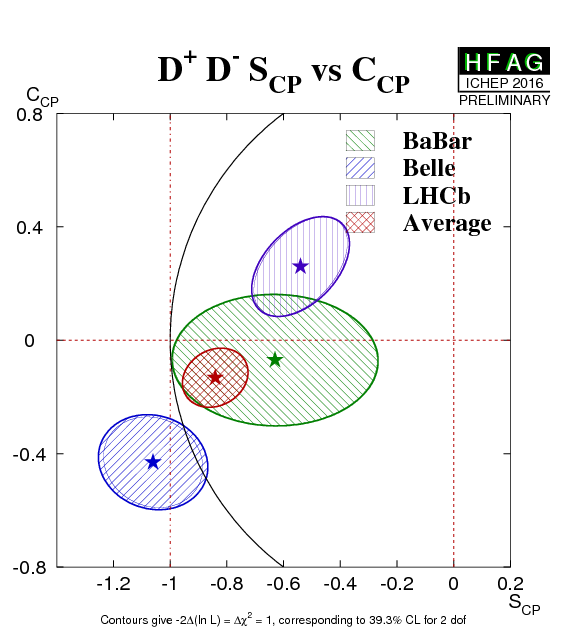
\includegraphics[height=7.5cm]{figs/D+D-S_CPvsC_CP.png} &
    \end{tabular}
  \end{center}
  \vspace{-0.5cm}
  \caption{\label{b2ddwa}World average of time-dependent $CP$ observables in $B^0 \to D^+ D^-$, reproduced from HFAG~\cite{HFAG}.}
\end{figure}

The BaBar and Belle Collaboration obtained the first observation of $CP$-violation
in the channels $B^0 \to D^{(*)}_{CP} h^0$, where $h^0$ is a light unflavored neutral
meson, by combining their final datasets \cite{babar_belle_D0h0}. Neglecting the
very small contribution from the $CKM$ suppressed amplitude $b \to u\bar{c}d$,
the time dependent analysis is sensitive to $\sin(2\beta)$. A joint likelihood,
sharing the same physics parameters but independent background modeling parameters,
the two experiments find:
\begin{eqnarray}
-\eta_f S & = & +0.66 \pm 0.10 (\mbox{stat}) \pm 0.16 (\mbox{syst}), \\
C & = & +0.02 \pm 0.07 (\mbox{stat}) \pm 0.03 (\mbox{syst}), 
\end{eqnarray}
with the significance of the observation beeing 5.4 standard deviations. 

\section{Measurements of the CKM angle $\gamma$}
\label{sec:gamma}
Measurements of the CKM angle $\gamma$ require the interference of $b\to u$ and $b\to c$ transitions.
Such interference can occur in the decays of charged as well as neutral $B$ hadrons, in tree-dominated
transitions as well as transitions where both tree and loop diagrams contribute.
The measurement of $\gamma$ from the tree-dominated decays of $B^\pm$ mesons, covered in the 
proceedings of WG5~\cite{WG5PROC}, has a particular importance as it allows a purely tree-level\footnote{Higher order box corrections~\cite{ZupanBrodGamma}
only enter at $\delta\gamma/\gamma \approx 10^{-7}$, well beyond any current or future experimental sensitivity.}
determination of the apex of the unitarity triangle, and therefore a test of the self-consistency of the CKM
mechanism of $CP$ violation when compared with determinations of $\alpha$ and $\beta$ in transitions where
both tree and loop diagrams contribute. It is also, however, possible to measure $\gamma$ by exploiting
$CP$ violation in the interference of mixing and decay of neutral $B$ mesons. These time-dependent determinations
of $\gamma$ are particularly powerful in the case of $B^0_s$ mesons, because the large width difference between
the light and heavy $B^0_s$ eigenstates makes additional $CP$ observables available compared
to the $B^0$ system and allows for a determination of $\gamma$ with fewer ambiguities. 
%While these are not
%strictly tree-level determinations, as the mixing of neutral $B$ mesons

A particularly powerful time-dependent measurement of $\gamma$, described in detail in these proceedings~\cite{DSKPROC}, utilizes the decay $B^0_s \to D^\pm_s K^\mp$.
In this case the $b\to u$ and $b\to c$ transitions are both of order $\lambda^3$, leading to large interference, and
the large value of $\Delta\Gamma_s$ allows for a determination of $\gamma$ with only a twofold ambiguity. 
The preliminary result obtained with the full Run~I LHCb dataset, which shows $3.6\sigma$ evidence for $CP$-violation in this mode, is
\begin{equation}
\gamma      = (127_{-22}^{+17})^\circ\,,\phantom{space}
\strong = (  358_{-16}^{+15})^\circ\,,\phantom{space}
\rdsk   = 0.37_{-0.09}^{+0.10}\,,\phantom{space}
(68.3\% \textrm{CL})\phantom{space}  
\end{equation}
\begin{equation}
\gamma      = (127_{-50}^{+33})^\circ\,,\phantom{space}
\strong = (  358_{-33}^{+31})^\circ\,,\phantom{space}
\rdsk   = 0.37_{-0.19}^{+0.19}\,,\phantom{space}
(95.4\% \textrm{CL})\phantom{space}  
\end{equation}
where $\strong$ is the $CP$-conserving angle between the $b\to u$ and $b\to c$ transitions,
$\rdsk$ is the amplitude ratio of the interfering diagrams, and the intervals for the angles are expressed modulo $180^\circ$.
The uncertainties are a combination of statistical and systematic ones; the statistical uncertainties dominate
and all systematic uncertainties are expected to scale with luminosity for the foreseeable future.

While not the most sensitive single-mode determination of $\gamma$, $B^0_s \to D^\pm_s K^\mp$ plays a similar
role in the overall LHCb combination~\cite{LHCb-PAPER-2016-032} of $\gamma$ to that of the GGSZ measurement. Because of their twofold ambiguity, these measurements
select the ``correct'' solution among the ones allowed by the most precise ADS/GLW measurement~\cite{LHCb-PAPER-2016-003}. For this reason the determination
of $\gamma$ from $B^0_s \to D^\pm_s K^\mp$, which is only possible at LHCb, will remain a key measurement for both the current
and upgraded LHCb detectors. LHCb is also pursuing a measurement of time-dependent $CP$-violation in
the decay mode $B^0 \to D^\pm \pi^\mp$, described in these proceedings~\cite{BDPIPROC}, but no results are available yet.
This measurement, previously performed by BaBar~\cite{Aubert:2005yf}, \cite{Aubert:2006tw} and Belle~\cite{Bahinipati:2011yq}, \cite{Ronga:2006hv}
is much less sensitive than $B^0_s \to D^\pm_s K^\mp$, both because of smaller interference and because
the small value of $\Delta\Gamma_d$ leads to fewer accessible $CP$-observables. The much smaller $CP$ asymmetry
also makes this measurement particularly sensitive the asymmetries in the flavor tagging of $B^0$ and $\bar{B^0}$ mesons.
Nevertheless, it is expected that both LHCb and Belle-II will carry out this measurement in the future.

\section{Conclusion}
The last two decades have seen an enormous progress in the understanding of $B$ meson mixing and mixing-related
$CP$ violation, both in terms of precise experimental measurements of the underlying constants of nature and in terms of 
the theoretical understanding of their values within the Standard Model. We now have precise measurements 
or stringent limits on the mass splitting, width splitting, and mixing phase in both the $B^0$ and $B^0_s$ systems,
while mixing-induced $CP$ violation is being precisely measured or constrained in an ever increasing number of final states.
With the LHCb upgrade~\cite{} and Belle~II~\cite{Abe:2010gxa} detectors due to come online in the next years, and none of the fundamental measurements
yet systematically limited, we can expect this progress to continue. Important contributions, particularly as regards
$\phi_s$ and $\Delta\Gamma_d$ can also be expected from CMS and ATLAS, and in particular it is realistic to expect the $B^0_s$ mixing
phase to be measured significantly away from zero even at the Standard Model value within the next decade. Recently
the LHCb collaboration has proposed a Phase~II upgrade of its detector~\cite{}, to take data in the HL-LHC period,
which would collect 300~fb$^{-1}$, and enable not only a single-experiment observation of $\phi_s$ in multiple independent
decay modes, but also make it possible to see evidence for a non-zero $\Delta\Gamma_d$ at its Standard Model value.
\textbf{ADD SOME WORDS ON THEORY TO FINISH THIS OFF}
%Particle physics is now roughly where the French monarchy was in 1788, and CERN is Versailles. But who will be our Robespierre?


%\bibliographystyle{PoS}
\bibliography{skeleton}


\begin{thebibliography}{99}

% I'm not citing this, but I put it here just in case
%\bibitem{atlas_phis_7TeV}
%  G.~Aad \emph{et al.} (ATLAS Collaboration),
%  \emph{Flavor tagged time-dependent angular analysis of the $B^0_s \to J/\psi \phi$ decay
%    and extraction of $\Delta\Gamma_s$ and the weak phase $\phi_s$ in ATLAS},
%  \emph{Phys.~Rev.~D} {\bf 90}, 052007 (2014) [{\tt arXiv:1407.1796 hep-ex}].

\bibitem{atlas_phis_8TeV}
  G.~Aad \emph{et al.} (ATLAS Collaboration),
  \emph{Measurement of the CP-violating phase $\phi_s$ and the $B^0_s$ meson decay width
    difference with $B^0_s \to J/\psi \phi$ decays in ATLAS},
  \emph{JHEP} {\bf 1608}, 147 (2016) [{\tt arXiv:1601.03297 hep-ex}].

\bibitem{cms_phis}
  V.~Khachatryan \emph{et al.} (CMS Collaboration),
  \emph{Measurement of the CP-violating weak phase $\phi_s$ and the decay width difference
    $\Delta\Gamma_s$ using the $B^0_s \to J/\psi \phi(1020)$ decay channel in pp collisions
    at $\sqrt{s}$ = 8 TeV},
  \emph{Phys.~Lett.~B} {\bf 757}, 97 (2016) [{\tt arXiv:1507.07527 hep-ex}].

  
\end{thebibliography}
  
\end{document}
